\documentclass[12pt,a4paper]{article}
\usepackage{biblatex}
\usepackage{times}
\usepackage{durhampaper}
\usepackage{amssymb}
%\usepackage{harvard}


%\newcommand{\testingbreak}{\pagebreak}%

\newif\iftesting
%\testingtrue

\newcommand{\testingbreak}{\iftesting \pagebreak \fi}%

\usepackage{psvectorian}

\newcommand{\ornamentleft}{%
    \psvectorian[width=2em]{2}%
}
\newcommand{\ornamentright}{%
    \psvectorian[width=2em,mirror]{2}%
}
\newcommand{\ornamentbreak}{%
    \begin{center}
        $\ast$~$\ast$~$\ast$
    \end{center}
}
\usepackage{mathtools}

\usepackage{listings}
\usepackage{xparse}

\usepackage{xcolor}

\usepackage{pifont}
\newcommand{\cmark}{\ding{51}}%
\newcommand{\xmark}{\ding{55}}%

\usepackage{booktabs}
\usepackage{multirow}

\definecolor{codegreen}{rgb}{0,0.6,0}
\definecolor{codegray}{rgb}{0.5,0.5,0.5}
\definecolor{codepurple}{rgb}{0.58,0,0.82}
\definecolor{backcolour}{rgb}{0.95,0.95,0.92}

\lstdefinestyle{mystyle}{
    backgroundcolor=\color{backcolour},   
    keywordstyle=\color{magenta},
    numberstyle=\tiny\color{codegray},
    stringstyle=\color{codepurple},
    basicstyle=\ttfamily\footnotesize,
    breakatwhitespace=false,         
    breaklines=true,                 
    captionpos=b,                    
    keepspaces=true,                 
    numbers=left,                    
    numbersep=5pt,                  
    showspaces=false,                
    showstringspaces=false,
    showtabs=false,                  
    tabsize=2
}

\lstset{style=mystyle}

\lstset{language=C, style=mystyle}

%\citationmode{abbr}
%\bibliographystyle{agsm}
\addbibresource{projectpaper.bib}

\title{TBD}
\author{} % leave; your name goes into \student{}
\student{qwrx21}
\supervisor{}
\degree{MEng Computer Science}

\date{}

\begin{document}

\maketitle

\begin{abstract}
ExaHyPE (``An Exascale Hyperbolic PDE Engine'') is a software engine for solving systems of first-order hyperbolic partial differential equations (PDEs).
Hyperbolic PDEs can be used to describe many physical phenomena such as earthquakes, fluid dynamics and gravitational waves.
This paper explores using a compiler based approach to generate fast compute kernels for the Finite Volume scheme, which can be used to solve PDEs within ExaHyPE.
Our compiler, \phlat, is used to generate Flat Long And potentially Transformed code, and aims to improve single core throughput.
Users describe their problem as a DAG (Directed Acyclic Graph), where every node is a primitive operation, or a DAG itself.
Then this highly nested structure is then flattened and transformed into code; we target C++.
Generated kernels are typically thousands of lines long.
We find these kernels out preformed current ExaHyPE kernels by $9\times$ to $16\times$.
We explore why conventional compilers, such as \texttt{g++}, can better optimise our compiled kernels, deducing that our compiled kernels can be better vectorized on SIMD architectures over hand optimised kernels.

\end{abstract}

\begin{keywords}
ExaHyPE
\end{keywords}

\testingbreak
\section{Introduction}
% PDEs - what they are
Many physical phenomena can be described by partial differential equations (PDEs) including:  seismic wave propagation \cite{earthquakePDE}, fluid dynamics \cite{exahype}, and relativistic astrophysics \cite{relativisticPDE}.
As such, PDE solutions can have an important real world impact by, for example, improving tsunami modeling \cite{tsunamiPDE}.


Analytical PDE solutions are challenging to derive, and general solutions for any initial conditions or boundary conditions do not exist.
Instead, we rely on numerical methods to calculate approximate solutions.
However, numerical methods are computationally intensive; increasing the size of the problem, or the accuracy of the solution, increases the computational work required.
Many real world problems require billions of degrees of freedom to model.
The sheer scale of these computations requires the use of high performance computing (HPC), where algorithmic advances and supercomputers make these problems tractable.

In HPC, there are 2 ways to increase computational throughput, either by using more hardware, or by using available hardware more efficiently.
Supercomputing hardware is ever improving, and exa-scale systems are on the horizon.
However, relying on more hardware runs into cost and availability issues.
Therefore, optimising code to better use the hardware is often preferable.
In HPC code there are many levels at which optimisation can occur, one of the most fundamental being improving the throughput of a single core.
There are many example in literature of this having a significant effect on the performance of HPC code \cite{YATeTo,seisolPFLOP,codegen_dg_SIMD}, and this will be the area of optimisation we explore.     

% Exhaype - what it is
Our focus will be on the per core performance of Finite Volume (FV) kernels used to solve PDEs within ExaHyPE (an Exascale Hyperbolic PDE Engine) \cite{exahype}.
Implementing a HPC FV solver is a non-trivial task, and can take research teams months, or even years \cite{tensorChemistry}.
This is the problem that ExaHyPE solves by providing a generalised framework to create solvers for many different problems.
ExaHyPE's domain is linear and non-linear hyperbolic systems of PDEs written in first order form.

The Peano framework \cite{PeanoFramework} lies at the heart of ExaHyPE.
This is responsible for dividing the spacial domain into smaller patches and distributing these patches across computing resources.
Every patch is updated by a single core using the FV scheme.
It is this update process we will optimise.

To use ExaHyPE, a user begins by describing their problem to the ExaHyPE toolkit using a Python interface.
A user will specify information such as: how many unknowns and auxillary variables are used; whether their problem uses a non-conservative product (NCP); what numerical scheme they want to use; if they want to use fixed or adaptive time stepping; how frequently the solution should be plotted; and more.
This is used by the ExaHyPE toolkit to generate a project.
This project is primarily populated by glue code that invokes ExaHyPE, however there are a few placeholder functions that need to be filed in by the user.
These placeholder functions are used to describe the PDE, calculating: flux, eigenvalues, initial conditions, boundary conditions, and non-conservative products (if applicable).
Upon completing these placeholder functions, the project can be compiled and run on systems ranging from a laptop to a supercomputer.

% Exahype - benifits of exahype (fast flexible, friendly)
ExaHyPEs is designed to be fast, flexible and user-friendly; allowing users to create fast programs to solve a wide range of problems while requiring minimal effort from the user.
However, being flexible and user friendly often limits the opportunities for optimistations, especially at the boundary between user and engine code.
In this paper we set out to solve this problem using our compiler based approach \phlat, so called for the Flat Long and potentially Transformed code it produces.
\phlat aims to bridge the gap in ExaHyPE between being flexible and friendly, while producing fast C++.  

\phlat{}'s approach to optimisation is to generate C++ that \texttt{g++}, \texttt{clang++}, \texttt{ipcx}, e.t.c. are more capable of optimising.  
Namely, \phlat can be used to generate monolithic functions that are tens of thousands of lines long.
In this paper we investigate the performance of these kernels and thus how well they are optimised by compilers.

Relying on the compiler for optimisations is often taken for granted, simply appending an \texttt{-O3} flag to the compiler arguments can increase the performance of code by orders of magnitude.
And using vendor specific compiler, like Intel's \texttt{ipcx}, offers code hardware specific optimisation.
As such, relying primarily on compilers for optimisation is a promising direction for exploration.
Also looking to the future, we see that compilers are only getting more advanced.
Most recently the application of Machine Learning within compilers is being explored \cite{compiler-ml-opt,lots-of-compiler-options}, and development environments such as CompilerGym \cite{compiler-gym} suggest this area of research is set to expand.
Thus suggesting that relying on compilers also offers an aspect of longevity to optimisations as well.

% what is in each section
In the next section we go into depth about what problem \phlat solves within ExaHyPE, followed by discussing similar compiler based approaches.
In Section \ref{sec:methodology} we explain the architecture of \phlat and how it is used to generate compute kernels.
In Section \ref{sec:results} we will discuss the performance of kernels generated along with the practicalities of using \phlat.

\testingbreak
\section{Problem Statement}
\subsection{Background}
Our focus will be applying the Finite Volume (FV) scheme to solve linear and non-linear hyperbolic PDEs in first order form.
We express these PDEs mathematically with the equation
% See exahype template
\begin{equation}\label{eq:non-lin-pde}
    \frac{\partial \mathbf{Q}}{\partial t}(x,t) + \nabla \cdot \mathbf{F}(\mathbf{Q}) + \mathbf{B}(\mathbf{Q}) \cdot \nabla \mathbf{Q}(x,t) = \mathbf{S}(\mathbf{Q})
\end{equation}
where $\mathbf{Q}(x,t)\subset \mathbb{R}^q$ is a time and space dependent state vector for any $x$ in our spatial domain $\Omega\subset \mathbb{R}^{d \in \{2,3\}}$ and $t>0$.
The number of conserved state variables, $q$, can vary from $5$ in the 3D Euler Equations, $58$ in the Einstien Relativity equations (CCZ4) \cite{CCZ4}.
$\mathbf{F}$ is the conserved flux vector, $\mathbf{B}$ the (system) matrix composing the non-conservative fluxes and $\mathbf{S}(\mathbf{Q})$ the source term.


We will derive the FV scheme for  (\ref{eq:non-lin-pde}) in the case that $B(Q)=S(Q)=0$
\begin{equation*}
    \frac{\partial \mathbf{Q}}{\partial t} + \nabla\cdot \mathbf{F}(\mathbf{Q}) = 0.
\end{equation*}
FV begins by dividing the spacial domain into finite volumes, known as cells.
For a cell, $i$, we take an integral over its volume $v_i$
\begin{equation*}
    \int_{v_i}\frac{\partial \mathbf{Q}}{\partial t}\,dv + \int_{v_i}\nabla\cdot \mathbf{F}(\mathbf{Q})\,dv = 0.
\end{equation*}
Then we integrate the first term to give the average state $\bar{\mathbf{Q}_i}$ over the cell, and apply divergence theorem to the second term
\begin{equation}\label{eq:fv-almost-done}
    v_i\frac{\partial \bar{\mathbf{Q}_i}}{\partial t} + \oint_{S_i}\mathbf{F}(\mathbf{Q})\cdot \mathbf{n} \, dS = 0
\end{equation}
where $S_i$ is the surface of cell $i$ and $\mathbf{n}$ is the outward facing normal vector.
Rearranging (\ref{eq:fv-almost-done}) for the time derivative we find
\begin{equation}\label{eq:fv-done}
   \frac{\partial \bar{\mathbf{Q}_i}}{\partial t} = -\frac{1}{v_i} \oint_{S_i}\mathbf{F}(\mathbf{Q})\cdot \mathbf{n} \, dS.
\end{equation}

If we select an simple geometry for our cell, squares/cubes are used in ExaHyPE, then calculating the 2D surface integral is simply a sum across the 4 faces of a square (or in 3D, the 6 faces of a cube).
Applying this calculation to (3) gives the time derivative of $Q$, which can then be used in a time stepping scheme such as explicit Euler to progress $Q$.
%This method can be generalised and applied to Equation \ref{eq:non-lin-pde}, to give the FV scheme used within ExaHyPE.  

\subsection{ExaHyPE}


% Can we make exahype better
% while not making it worse
\newcommand{\proc}[1]{\textbf{#1}}

% we will focus on patch update
An ExaHyPE project is a majority of engine code, and a small amount of user code which is used to describe the PDE.
The interface between the engine and user code is built on the patten of passing function pointers of user functions to engine code.
Here is an example:
\begin{lstlisting}[language=c]
void engine_function(std::function<...> user_function){
    // ... Do something
    val = user_function();
    // ... Use the value of the user function 
}

void engine_core(){
    auto user_func = project::user_land::foo;
    engine_function(user_func);
}
\end{lstlisting}

This patten is good design practice, as it completely decouples engine functions from user functions, apart from at a single crossover point.
Thereby allowing the engine to be developed in isolation from user codes, and allowing the engine to support any user codes that respect the required function signatures.
However, this patten, and the total disconnect between user and engine code it allows, is not without its disadvantages, as we will discuss.

Our focus will be on the \proc{Patch Update} process.
This process is heavily reliant on user code, and as such dominates the runtime of user code.
Furthermore, for arithmetic intense PDEs, this process dominates the entire running time of an ExaHyPE program.
We will begin by explaining the \proc{Patch Update} process.
Then proceed to highlight inefficiencies within this process. 

The smallest unit of space in a FV scheme is a cell.
Algorithmically a cell is an array of \lstinline{double} that store the state of that cell.
As mentioned previously the size of the state vector can vary from $4$ values to over $40$.
Cells are then grouped up into a patch.
Within ExaHyPE, patch data is stored in a AoS (Array of Structures) form.
Patch sizes are typically 3x3 cells in 2D or 3x3x3 cells in 3D.
The size of patches can be adjusted by a user, say to 5x5, however a patch size is a constant throughout the runtime of the program.
Within ExaHyPE, the Peano Framework \cite{PeanoFramework} is responsible for splicing the spacial domain into patches, and distributing patches across compute nodes and compute threads.
As such, we are concerned with the single threaded process of \proc{Patch Update}.
\proc{Patch Update} is used to evolve the values of cells in a patch by a given timestep.
This is done by applying source terms to the cells, then calculating flux and non-conservative products (NCP) for every face of a cell and applying it to the cells state.
As a technical detail, to evaluate every face of every cell in a patch we require a halo of cells as demonstrated in Figure \ref{fig:patch}.

\begin{figure}[h!]
    \begin{center}
        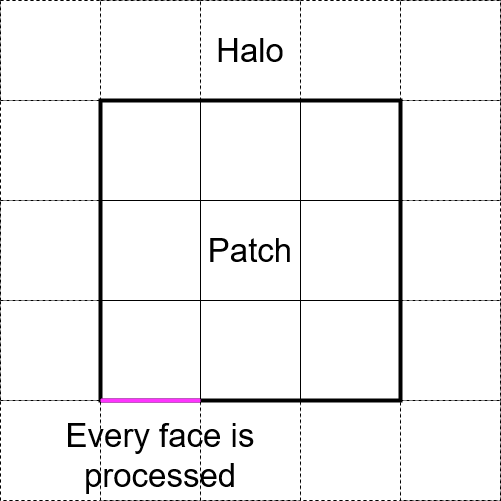
\includegraphics[width=.2\textwidth]{patch.png}
        \caption{Example of a 3x3 patch, with a halo of cells.}
        \label{fig:patch}
    \end{center}
\end{figure}


In summary, \proc{Patch Update} is a function whose input is: a haloed patch; a timestep; and patch meta-data such as its size in space. And whose output is: the patch (without a halo) that has been progressed in time. 

Calculating the flux and NCP at a shared face between 2 cells a non-trivial task.
This is because the face is at a discontinuity between the states of the 2 cells, and is known as the Riemann problem in FV.
As such, we require a scheme to solve the Riemann problem, which we will call the \proc{Numerical Ingredient}.
Many such schemes exist, such as Upwind and Downwind schemes, and the correct scheme to use depends on the problem.
Within ExaHyPE the Rusanov scheme \cite{rusanov} is used by default, as it well serves the role of a general \proc{Numerical Ingredient}.
The \proc{Numerical Ingredient} has an input of 2 cells and meta data about the face (e.g. its position in space).
And outputs 2 state vectors describing the change of state experienced by each cell.

At the bottom level of this hierarchy we have the \proc{Problem Descriptions}.
These are a collection of user defined functions the calculate: flux, NCP, source terms, and maximum eigenvalues.
All these functions share a similar input interface, taking single cell and the meta data for that cell.
And they output either a state vector or single value, depending on what quantity they are calculating.
In the default ExaHyPE setup, it will be \proc{Patch Update} that calls the source term function.
And \proc{Numerical Ingredient} that calls the flux, NCP and max eigenvalue functions.

A summary of the abstraction hierarchy of \proc{Patch Update} can be found in Table \ref{tab:patch_update}

\begin{table}
\begin{tabular}{lllcc}
    \toprule
    Process & User/Engine &Uses Functions & Input Size & Output Size\\
    \midrule
    \proc{Patch Update} (\proc{PU})&Engine& \makecell[l]{\proc{NI}, \proc{PD}\\ (source term)} & $q \cdot (p+2)^d+m$ & $q\cdot p^d$\\
    \proc{Numerical Ingredient} (\proc{NI}) &\makecell[l]{Engine \\(default),\\ User}& \makecell[l]{\proc{PD} (flux, ncp,\\ max eigenvalues)} & $2q+m$ & $2q$\\
    \proc{Problem Descriptions} (\proc{PD}) & User& - & $q+m$ & $q$ or $1$\\
    \bottomrule
\end{tabular}
\caption{A summary of the level of abstraction within the \proc{Patch Update} function. $p$ is the number of cells along 1 dimension in a patch, $d$ is the dimension of the patch, $q$ are the number of state variables, $m$ is the size of patch/state metadata.}\label{tab:patch_update}
\end{table}

Now we have an understanding of \proc{Patch Update} we can investigate some of the potential performance issues it experiences.
% ISSUE: lambda functions, not inline
Firstly, as mentioned at the beginning of this section, ExaHyPE implements the function pointer pattern to interface between user and engine code.
As such, the definition of \proc{Patch Update} looks like this:
\begin{lstlisting}[language=c]
void full_numerical_ingredient(
    std::function<...> flux, std::function<...> ncp,
    /* other args */);
void full_patch_update(
    std::function<...> numerical_ingredient, std::function<...> source_term,
    /* other args */);

void engine_core(){
    std::function<...> numerical_ingredient = [&](/*other args*/){
        full_numerical_ingredient(
            user_land::flux, user_land::ncp, /* other args*/
        );
    };
    std::function patch_update = [&](/*other args*/){
        full_patch_update(
            numerical_ingredient, user_land::source_term, /*other args */
        );
    };

    patch_update(double * in_patch, double * out_patch, ...);
}
\end{lstlisting}
This is non-trivial to fully inline, hence there is the potential the compiler choices to make function calls.
However, function calls hinder vectorization, therefore this code may not be vectorized well.


% ISSUE: heap allocation
The next issue we encounter is the use of heap allocation.
The implementation of \proc{Patch Update} allows us to use a single function for many different user codes.
However, this also means algorithmic precautions must be take to safely handel any user codes.
Within both \proc{Patch Update} and \proc{Numerical Ingredient} temporary variables are used to receive the result of function calls.
The size of these temporary variables depend on the size of a cells state.
Hence, safe behaviour dictates that these temporary variables are declared on the heap as opposed to the stack, which is slow. 


% ISSUE: branching
% MAYBE ISSUE: consts as function arguments



% ISSUE: repeated + unused comp
The final issue we will acknowledge is the existence of repeated and unused computations.
As we saw, every functional call within \proc{Patch Update} takes a meta data argument.
Some of this meta data needs to be calculated for every function call.
For example, \proc{Numerical Ingredient} requires the coordinates for the center of the face it is processing.
These coordinates are calculated using the coordinates of the 2 cells that share this face.
However, \proc{Numerical Ingredients} such as Rusanov use this coordinate.
Hence, we run the risk of the compiler not eliminating this redundant computation, especially as its definition and usage lie across different functions. 
Beyond unused computation, there can also be repeated computation.
If we look at using Rusanov as our \proc{Numerical Ingredient} there are many repeated computations.
To calculate the flux at the shared face of 2 cells $a,b$ Rusanov calculates $flux(a), flux(b), max\_eigenvalue(a), max\_eigenvalue(b)$.
The flux at the face is then a function of these 4 values.
If we were to then calculate the flux between $b,c$ note that the computation of $flux(b), max\_eigenvalue(b)$ is repeated.
It may be challenging for the compiler to spot this repetition, especially as it again lies across multiple different functions.
Furthermore, \proc{Patch Update} cannot be optimised to take advantage of this property of Runsnov, as it would no longer work with any \proc{Numerical Ingredient}.

To summarize, \proc{Patch Update} has the constraint of supporting any \proc{Numerical Ingredient} or \proc{Problem Description}. 
Within \proc{Patch Update} the function pointer patten and safe behaviour such as heap allocation is used to meet this constraint.
However, this constraint is in contension with performance.
Although optimisations can be made for specific pairings of \proc{Numerical Ingredient} and \proc{Problem Description}, there is limited scope for general optimisations. 
And at the end of the day, case by case optimisation detracts from the draw of using a PDE engine in the first place.

It is desirable to use a technique that maintains the modularity of \proc{Patch Update} but increases potential for optimisation.
This is what we will explore, applying a compiler based approach to achieve these goals.



\testingbreak
\section{Related Work}
% Exahype templating
% make mroe systems, less user friendly


% Euler 3D SIMD speedup 1.04
% CCZ4 1.27

Much of ExaHyPE's code generation is preformed via templating.
Templating is a powerful, yet simple method to generate large sections of glue code.
Although as discussed in section \ref{sec:problem_statement}, templating along the boundary of user and engine code leaves opportunities for improvements.  
A solution to this problems was proposed by \citeauthor{templateExahype} by extending the domain of templating to user code \cite{templateExahype}.

\citeauthor{templateExahype} observed that while creating an ExaHyPE projects there are often 3 separable roles preformed by users.
These are: application experts, who focus on configuration of ExaHyPE; algorithm experts, who understand and implement the PDEs; and optimisation experts, who work at a lower level to increase performance.
The idea behind further templating is to allow these roles, which may be fulfilled by different people, to operate synergistically.
Increased templating also offers a convenient way to implement architecture aware optimisations, increasing code portability and speed.
\citeauthor{templateExahype} showed an example use case of their technique that applied a SIMD friendly SoA to AoS transformation to user code.
This transformation was tested on 2 problems: the Euler equations in 3D, and the Einstein equations from relativistic astrophysics (CCZ4).
They found that the memory bound Euler 3D problem experienced a $1.05\times$ speedup and the compute bound CCZ4 equations experienced a $1.27\times$ speedup.

While templating serves a vital role within ExaHyPE, we do not believe it to be the best way to optimise user code.
Templating inherently requires an optimisation expert for any performance improvements to be realized.
Our compiler based approach is based on the idea that conventional compilers are exceptionally powerful, and they should take the role of optimisation expert, not a person. 



% Yateto used a compiler
YATeTo (Yet Another Tensor Toolbox) \cite{YATeTo}, shares a similar philosophy to this paper, however YATeTo's approach relies on GEMM (General Matrix-Matrix Multiplication) libraries wheras we rely on conventional compilers alone.
YATeTo operates in the domain of linear hyperbolic PDEs, in partial, it is part of the Seisol project \cite{seisolPFLOP}, which focuses on applying the linear elastic wave HPDE to model seismic activity.
Although, YATeTo can be used for more general applications.

The Discontinuous Galerkin method often used to to solve HPDEs can, in the linear case, be discretized into a series of Tensor contractions.
YATeTo offers a Domain Specific Language (DSL) within python for users to describe their tensor contractions.
Then through a series of compilation steps outputs C++, which crucially contains many calls to GEMM libraries.
Highly performant GEMM libraries and BLAS (Basic Linear Algebra Subprograms) libraries are often distributed by system vendors.
These libraries are optimised for a wide range of input problems sizes, and often include hardware specific optimisations like improved cache usage.
It is unlikely that a user of these libraries could write code that was more performant than the library, and even if they could they would have to write new code for every system they used.
Hence, utlizing GEMM libraries can drastically speedup code.

Furthermore, YATeTo preforms optimisations within its compilation steps, such as strength reduction, sparsity patten exploitation and memory layout optimisation.
Overall, YATeTo achieved a speedups between $1.1\times$ to $6.5 \times$ within SeiSol, which is impressive.
YATeTo shows that automation of the optimisation process using a compiler can be very effective.
Especially while using high performance, system agnostic libraries such as GEMM.
Unfortunately, the use of tensor contractions cannot be carried over to non-linear HPDEs, due to their non-linearity.
Hence, we explore the more general technique of leveraging conventional compilers.   



% firedrake used a compiler
% Hummm
%\cite{FiredrakeAndCOFFEE}


%Auto code gen
% SIMD - problem specific
Although, YATeTo is not alone in the space of automatic optimisations using a compiler based approach.
\citeauthor{codegen_dg_SIMD} explore a similar linear domain as YATeTo in their paper that addresses optimising for modern architectures \cite{codegen_dg_SIMD}. 
However, their approach differs from YATeTo, as they choose to preform SIMD vectorisation within their compiler, introducing SIMD intrinsics to the output code, as opposed to YATeTo which uses GEMM libraries.
\citeauthor{codegen_dg_SIMD} state that there are 2 paths to introduce vectorisation within code.
Automatic vectorisation through conventional compilers, and explicit vectorisation where SIMD instrisic instructions are introduced by developers.
They argue that although the former is preferable, the latter will likely be more performant due to a developers problem specific knowledge.
As such, they introduce a compiler architecture that automatically preforms explicit vectorisation, using observations and deductions that arise from the tensor decomposition of linear HPDEs.

Again, our requirement of supporting non-linear HPDEs prohibits us from exploiting tensor contractions, and instead exposes us to a more varied range of inputs.
As such, we choose to use the former of  \citeauthor{codegen_dg_SIMD} path to vectorisation, relying entirely on conventional compilers to automatically vectorize our code.
However, this paper does show that users of \phlat may wish to explore the use of explicit techniques and problem specific knowledge to improve the performance of their programs.
Hence, as a design requirement \phlat should support this.
\citeauthor{codegen_dg_SIMD} found that their explicit vectorisation achived 50\% peak floating point performance solving the diffusion-reaction Equation on an Intel Haswell system.
Although, they noted that there was potential for further performance improvements with addition tweaking.  



\testingbreak
\section{Solution}

\newcommand{\vecc}[1]{\vec{\mathbf{#1}}}

\subsection{Overview and Domain Reduction}
% Overview
%   - we make a compiler
% for a restricted problem domain
% we generate a large amount of code
% we replace the lambda function with a call to this code
% pure functions with numerical input
% ignore the effects of numerical machine precision
Our solution will be a domain specific compiler that generates code for a conventional compiler e.g. g++ to optimise and turn into machine instructions.
We can define our goals for the compiler as follows:
\begin{itemize}
    \item Supports a large range of problems
    \item Generates code that is faster than the current default code
    \item Provides a user friendly interface for entering problems
    \item Practical to use (e.g. compile times are not too long)
\end{itemize}
To meet these goals it is first important to define the domain in which our compiler operates.

PDEs are mathematical functions.
Hence, we expect that all the substeps of solving PDEs are also mathematical functions.
This is certainly true in the FV scheme.
Looking at our main focus, the patch update step, we can say $\vecc{Q}_{out} = f(\vecc{Q}_{in}, t, dt, \vecc{x}, \vecc{dx})$ where
$\vecc{Q}_{in}$ and $\vecc{Q}_{out}$ are the input and output state of a patch,
$t$ is time,
$dt$ is the time step,
$\vecc{x}, \vecc{dx}$ are vectors describing the current patch's position and size, and $f$ is the patch update function.
Likewise, the numerical method and problem definitions can also be described as mathematical functions. 
Consequently, we can make the assertion that our compiler only needs to support pure functions.
This a useful restriction as it allows us to consider each function isolation, without the complication of side effects.

Our next observation is that mathematical functions accept a fixed length input and produce a fixed length output.
For example if $f$ is defined for $|\vecc{Q}_{in}|=100$ then the behaviour of $f$ on $|\vecc{Q}_{in}|=101$ is undefined.  
This eliminates the possibility of varying length inputs and outputs, again simplifying our compilers domain.
Further to this observation, every input and output is a real number.
We choose this to mean that all inputs and outputs are restricted to \texttt{double}.
This restriction could be relaxed to allow the use of all numerical data types e.g. \texttt{float}, \texttt{int} but will be left inplace to reduce the compiler complexity. 

% mby somethingg about how x/3/3/3 == x/3^3

Finally we add the restriction that control flow is not supported.
At first this may appear to be too hash of a restriction which imposes a serious limit on the compilers capabilities.
However, as we will discuss in Section \ref{sec:DAG} a majority, if not all, control flow can be hoisted to DAG (Directed Acyclic Graph) creation as it is not a fundamental feature of the mathematical functions, hence this restriction is a non-issue.
An exception to this are peicewise functions e.g.
\[
    y = \begin{cases} g(x)  & \text{if } x<0.5 \\  h(x)  & \text{if } x\geq 0.5 \\\end{cases}
\]
This will not be supported by the compiler.

As will be described in the next section, the computation is input as a DAG.
We can use this as an alternative definition of \phlat{}'s domain.
Any problem that can be represented as a DAG is within \phlat{}'s domain.




\subsection{DAG} \label{sec:DAG}
% What is a DAG - chip model
% [ ] Explain chip model
% [ ] Show example
% [ ] Control flow hoisting

\phlat begins with a Directed Acyclic Graph (DAG) as an input.
Currently it is the responsibility of a user to create such a DAG, however it would be entirely possible to generate a DAG using a user friendly format such as from a SymPy \cite{sympy} formula.
The DAG model we propose takes inspiration from hardware design languages.

In a hardware design language you define electrical components.
Each component has input and output ports and its output is a function of its input.
Furthermore, it is common place to see specifications and test cases along side a component to be used in verification.

In our DAG every node has a set of input and output ports.
Every input port must receive single value and every output port can transmit copies of a single value.
Every node $n$ in our graph describes a function: $\vecc{out ports}=n(\vecc{in ports})$ with the number of inputs and outputs being of a fixed length.

A node may be primitive and directly map to a primitive code operation, for example an addition node maps to $out_1 = in_1 + in_2$ (see Figure \ref{fig:bin_add}).
Or a node may be composite, where it is a DAG itself.
Composite nodes would map to functions in the final code output.
Figure \ref{fig:bn} demonstrates composite nodes with the calculation $out_0 = (in_0)^3 + in_1$ where the function \textit{cubed} has been implemented as a subgraph.
The nested structure that provided by composite nodes gives the DAG model a lot of expressive power and modularity.
For example, a user can create Problem Definition DAGs, then hand those DAGs to pre-made \proc{Patch Update} and \proc{Numerical Ingredient} DAG builders to create a DAG that describes the full \proc{Patch Update} process.


\begin{figure}[h!]
    \begin{center}
        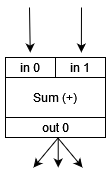
\includegraphics[width=.15\textwidth]{binary_add.png}
        \caption{Example of binary addition as a DAG node.}
        \label{fig:bin_add}
    \end{center}
\end{figure}

\begin{figure}[h!]
    \centering
    \subcaptionbox{Top level\label{fig:bn1}}{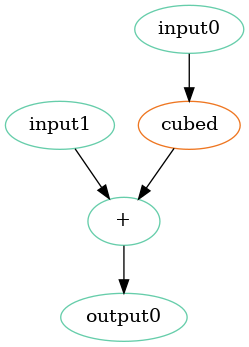
\includegraphics[width=.2\textwidth]{basic-nested-part1.png}}
    \hspace{1em}
    \subcaptionbox{Exploded view\label{fig:bn0}}{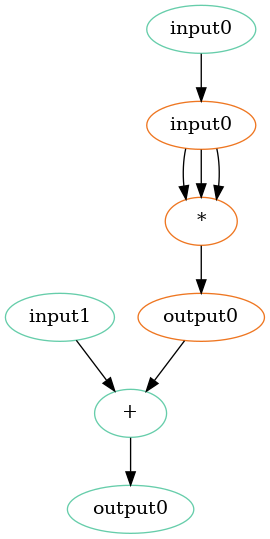
\includegraphics[width=.2\textwidth]{basic-nested-part0.png}}
    \caption{Example of a nested DAG that calculates $out_0 = (in_0)^3 + in_1$. The colour of a node is used to show if that node is composite or part of a composite node. NOTE. the visualisation displays a node's input edges in a random order.}\label{fig:bn}
\end{figure}

Provided that the graph is acyclic we can always find an order to evaluate every node in the graph for some given input.
In \phlat every DAG node implements an \texttt{eval} function which takes its inputs as a list and returns the outputs as a list.
The \texttt{eval} function allows us to test every DAG we define using unit and integration tests.

DAGs are created in python.
Every node type is a class.
To create a node you create an object from the class of node you desire.
DAGs are a special class of node that implement additional functions.
Namely, DAG nodes store a sparse definition of the graph they represent and provide an interface for users to add edges to the graph.
The \texttt{eval} functions of all the primitive nodes are simple, often only preforming one operation.
The \texttt{eval} function for a DAG node is more complex, first calculating a valid traversal order of the DAG.
Then following this traversal order, the DAG node calls the \texttt{eval} function on each subnode, forwarding the output of completed \texttt{eval} to the input of nodes yet to be processed.
This process repeats until the entire DAG has been traversed.

Using python to create DAGs allows for the hoisting of control flow.
For example, take the a flux function used in an ExaHyPE project:
\begin{lstlisting}[language=c]
void flux(
  const double * __restrict__ Q, // input
  ...
  int normal,
  double * __restrict__ F // output
)  {
  switch(normal){  
  case 0: //in x direction
	  F = flux_x(Q, ...)
	  break;
  case 1: //in y direction
	  F = flux_y(Q, ...)
	  break;
  }  
}
\end{lstlisting}
The switch statement is run every evaluation of flux and depends on the value of the normal.
However, in \proc{Patch Update} the value the normal is known at compile time.
Therefore, we can use a builder patten in python to hoist this control flow out of the flux function.
\begin{lstlisting}[language=python]
def build_flux_DAG(normal:int)->DAG:
    if normal==0:
        return build_flux_x()
    else:
        return build_flux_y()
\end{lstlisting}




\subsection{IR}
% What is the IR - llvm inspired
% [ ] Explain IR
% [ ] Show example


DAGs are an powerful and expressive way to represent an input problem, however code generation directly from a DAG is challenging.
To overcome this issue we introduce an intermediate representation (IR).
The goal of this IR is to offer a middle ground between the DAG and output code.
It should be easy to transform the DAG into an IR, and it should be easy to transform this IR into code.
The IR we use takes inspiration from LLVM.
It is a set of function definitions, and within each function definition there is a linear sequence of instructions.

One of the main challenges we came across during the code generation process was variable management.
Our compiler supports interchangeable code generation backends, allowing different languages to be targeted.
This means it's preferable to include information such as variable declaration and complex function signatures in the IR, allowing code generation backends to stay as slim as possible.
However, the complications induced by variable declarations and function signatures are a key reason why code generation directly from a DAG is hard.   


To combat these opposing requirements we create 2 standards for our IR.
The IR can be \textit{loose}, and the IR can be \textit{tight}.
When we transform our DAG we transform it into a loose IR.
A loose IR doesn't worry about variable declaration, variable declaration is implicit like in python.
There are also useful tools available in loose IRs such as a special class of temporary variables.
Additionally, loose function signatures are kept very simple.
A loose function maintains a list of (possibility hundreds) of single value input variables and a list of (possibly hundreds) of single value output variables.
The relaxed nature of the loose IR makes it ideal for preforming transforms (such as for optimisations) as there are few ways to invalidate a loose IR.

On the other hand, a tight IR is much stricter.
In a tight IR all variable must be named and declared.
And a tight function signature mirrors that of the target output code, containing a mixture of input and output variable that can be single values or arrays.
Figure \ref{fig:tight_loose} provides an example of loose and tight IR. 

\newsavebox{\looseIRlisting}
\begin{lrbox}{\looseIRlisting}% Store first listing
\minipage{.68\textwidth}
\begin{lstlisting}
define VOID @kernel (%in0, %in1) (%out0, %out1):
	%tmp1 = %in0
	%tmp2 = %tmp1 * %tmp1 * %tmp1
	%tmp3 = %in1
	%tmp4 = %tmp2 + %tmp3
	%tmp5 = %tmp4
	%tmp6 = %tmp2 - %tmp3
	%tmp7 = %tmp6
	%out0 = %tmp5
	%out1 = %tmp7
\end{lstlisting}
\endminipage
\end{lrbox}

\newsavebox{\tightIRlisting}
\begin{lrbox}{\tightIRlisting}% Store first listing
\minipage{.68\textwidth}
\begin{lstlisting}
define VOID @kernel (new #list(in), new #list(out)):
	new #tmp2 = #in[0] * #in[0] * #in[0]
	#out[0] = #tmp2 + #in[1]
	#out[1] = #tmp2 - #in[1]
	<return nothing>
\end{lstlisting}
\endminipage
\end{lrbox}

\begin{figure}
\centering

\sbox{\measurebox}{%
  \begin{minipage}{.68\textwidth} \centering
        \subfloat[Loose IR]{\label{fig:figB}\usebox{\looseIRlisting}}
        \vspace{1em}
        \subfloat[Tight IR]{\label{fig:figC}\usebox{\tightIRlisting}}
  \end{minipage}
}

\usebox{\measurebox}\qquad
    \begin{minipage}[][\ht\measurebox][c]{.26\textwidth}
      \subfloat[Input DAG]{\label{fig:loose_tight_dag}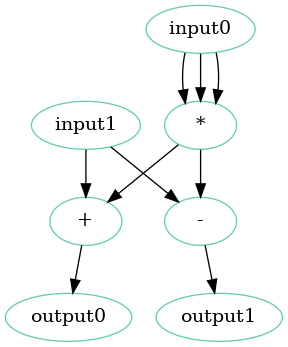
\includegraphics[width=\textwidth]{tight_vs_loose.png}}
       
    \end{minipage}
\caption{Example of the difference between a loose IR and tight IR. Figure \ref{fig:loose_tight_dag} shows the corresponding input DAG.}
\label{fig:tight_loose}
\end{figure}


\subsection{Compiler Architecture}
Our compiler consists of 3 stages.
The DAG transform stage, the IR transform stage, and the code generation stage.

% DAG Transforms
In the DAG transform stage a series of user specified transforms are applied to the DAG.
The most useful of these transforms is the flatten transform.

\begin{figure}[h!]
    \centering
    \subcaptionbox{Nested DAG}{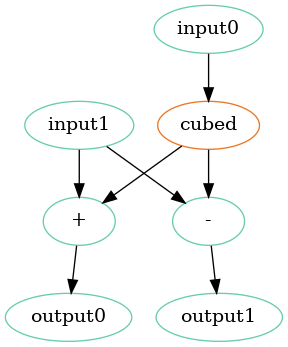
\includegraphics[width=.2\textwidth]{flatten-part1.png}}
    \hspace{1em}
    \subcaptionbox{Exploded view of nested DAG}{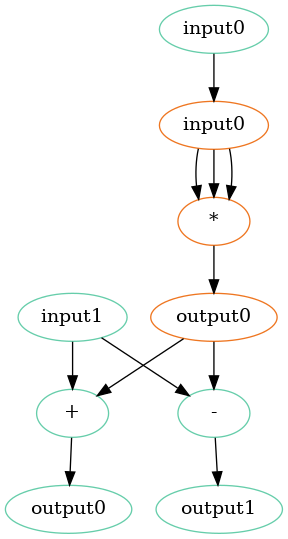
\includegraphics[width=.2\textwidth]{flatten-part0.png}}
    \hspace{1em}
    \subcaptionbox{Flattened DAG}{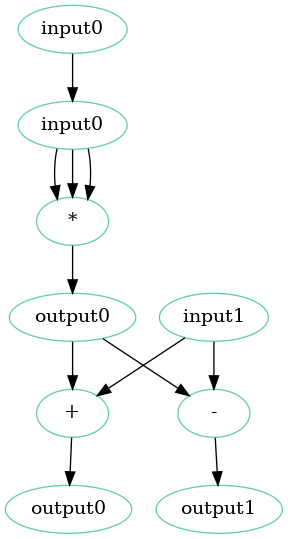
\includegraphics[width=.2\textwidth]{flatten-part2.png}}
    \caption{Example of the DAG flatten operation. Colours are used to indicated depth of nodes. Blue = depth 0, Orange = depth 1.}\label{fig:flatten_example}
\end{figure}

This transform takes a nested DAG (i.e. a DAG containing composite nodes) and for every composite node, the composite node is deleted and replaced by a copy of the DAG contained within the composite node.
Applied recursively, a highly nested DAG can be reduced to only contain primitive nodes, i.e. it is flattened.
This transform causes the final output code to be a single monolithic function, as opposed to a function containing many function calls.
An example of the flatten transform can be found in Figure \ref{fig:flatten_example}

Another notable transform we investigated was the removal of duplicated computation.
Within a DAG, duplicate computation manifests itself as 2 equivalent nodes (e.g. 2 addition nodes) that share the same inputs.
Once 2 such nodes are identified one can be deleted, and its output edges copied over to the node that remains.
Some care has to be taken if an operations is commutative (e.g. addition and max) or not (e.g. subtraction and division).
This is an example of a user transform, as it is not necessary for the compiler to function.

% DAG -> IR
Once all the DAG transforms are completed the DAG is transformed into the IR.
To do so, the DAG and every sub-DAG are identified and processed separately creating a set of loose functions.
Processing a DAG begins by creating a valid traversal order, much like DAG \texttt{eval} does.
Then following this order, every node in the DAG is transformed into an IR symbol.
Primitive nodes map to equivalent primitive IR Symbols and composite nodes map to loose IR function calls.
The output of every port of every node is stored as a new temporary variable, and these temporary variables are passed as the input to other nodes.
At the end of the transform we have an IR in loose form.

% IR Transforms 
The second stage of \phlat is the IR transform stage.
Much like we apply a series of user defined DAG transforms, so to do we apply a series of user defined IR transforms.
Interestingly there are equivalences between DAG transforms and IR transforms.
For example, the DAG transform \texttt{Remove Passthrough Nodes}, which removes all the primitive nodes that simply pass through a single value, is approximately equivalent to the IR transform \texttt{Remove Forward Aliasing}, which removes all lines that look like \lstinline{%tmp_x=%tmp_y} (i.e. a line that copies a single value).
However, it is not the case that all IR and DAG transforms share this equivalence.
For example, in the IR you can create transforms to arrange a programs memory layout, but in a DAG there is no concept of memory layout.

% Loose IR -> Tight IR
%   - variable model
%   - function stencil 
Once the user defined IR transforms are applied the IR is transformed into a its tight form.
This process begins by applying user defined function signatures to loose IR functions, these are called function stencils.
This transforms all loose functions and function calls into tight functions.
A function function stencil consists of 3 parts: the desired arrangement of arguments in the tight function; a map from input variable to variable in the function argument; and a map of output variable to function arguments.

Once function stencil are applied, every temporary variable is replaced with a named variable.
A named variable is any variable that has a unique name and can be generated into code e.g. a normal variable and an array element.
The distinction between temporary variables and named variables may seem like unnecessary bloat, however it does serve an important propose.
Users may choice to create transforms that arrange their programs memory layout, for example targeting a SIMD friendly layout.
To do so they will replace temporary variables with named variables.
As it is not expected that users will tackle memory layout this transform creates a new normal variable for every temporary variable. 

The finally all the named variables are defined, creating a tight IR.
For the most part this involves defining a variable the first time it is observed.
However, special care is required for variables that are defined in the function signature and also for elements of arrays.

% Tight IR -> Code
The final step of \phlat is to transform the tight IR into code.
\phlat supports interchangeable code generation backends (CGB), however we have only implemented a C++ backend.
Within the C++ CGB we use the cparser python package.
The cparser package defines AST nodes (Abstract Syntax Tree) for C, and given an AST can generate code.
This reduces the problem of code generation to a problem of transpilation from the IR AST to a C AST.
This can be achieved with a post order traversal of the IR AST, generating C AST nodes from each of the IR AST nodes.
Finally, some post processing is preformed to transform the C into C++.
For example, the required standard library headers are inserted, and variable decorators such as \lstinline{__restrict__} are added.  

\subsection{Using \phlat to Generate Compute Kernel}
Using \phlat we can generate a compute kernel that preforms \proc{Patch Update}.
A user begins by creating DAGs of their \proc{Problem Definition}, using the builder patten (creating a function that returns a DAG).
DAGs can be tested using the \texttt{DAG.eval}, to ensure validity.
These DAG builders can then be passed to pre-existing \proc{Patch Update} and Rusanov DAG builders.
A user provides DAG builders instead of DAGs directly for 2 reasons.
Firstly, it allows them to hoist any control flow.
Secondly, this allows a new DAG to be built for every use of a user function.
 
The final output of the \proc{Patch Update} builder is the compute kernel DAG, which will contain many copies for the \proc{Numerical Ingredient} and \proc{Problem Description} DAGs.
This DAG is then passed through \phlat, where it undergoes DAG transforms, a DAG to IR transform, IR transforms, and finally code generation.
Users have the option to provide additional DAG or IR transforms.
The code is now ready to replace the old \proc{Patch Update} within ExaHyPE.
The most notable step of the default transform chain is the DAG flatten transform that turns many nested DAGS into a single flat DAG.
This transform is responsible for \phlat's characteristic compute kernels which are: Flat, Long (And potential Transformed).
Typically compute kernels will be thousands to tens of thousands of lines long, and contain no function calls.   

\testingbreak
\section{Validity}
\input{Sections/validity}

\testingbreak
\section{Results}
We used 3 test problems: Euler Equations in 2D and 3D (Euler 2D, Euler 3D), and the shallow water equations (SWE).
These 3 problems are provided as examples within the ExaHyPE repository, and those kernels were used as control kernels which we refer to as \textit{default}.
We then recreated these kernels as DAGs and used FLAT to compile them into C++.
Our first method for comparison is a simple synthetic benchmark that measured how many iterations per second a kernel could preform on a fixed input.  

\begin{table}
    \centering
    \begin{tabular}{lllrr}
\toprule
Problem & Kernel & System & Iterations per ms & Speedup \\
\midrule
Euler 2D & default & Intel & 152.90 & - \\
Euler 2D & compiled & Intel & 2486.15 & 16.26 \\
Euler 3D & default & Intel & 50.20 & - \\
Euler 3D & compiled & Intel & 603.29 & 12.02 \\
SWE & default & Intel & 150.98 & - \\
SWE & compiled & Intel & 2313.76 & 15.32 \\
Euler 2D & compiled & AMD & 3150.51 & 8.66 \\
Euler 3D & compiled & AMD & 663.42 & 8.62 \\
SWE & compiled & AMD & 2874.82 & 11.38 \\
\bottomrule
\end{tabular}
 
    \caption{Performance of compiled kernels against default kernel in a synthetic benchmark.} 
\end{table}

Our compiled kernels preformed well, achieving approximately an order of magnitude speedup over the \textit{default} kernels.
This translated to a \textbf{speedup of 5\% - 15\% in ExaHyPE}, which was to be expected for our memory bound test problems.

We also compared a hand optimised kernel against a compiled kernel. 
\begin{table}
    \centering
    \begin{tabular}{lrrr}
\toprule
Kernel & Iterations per ms & Speedup vs Default & Speedup vs Handmade \\
\midrule
default & 363.67 & 1.00 & 0.27 \\
handmade & 1364.63 & 3.75 & 1.00 \\
compiled & 3150.51 & 8.66 & 2.31 \\
\bottomrule
\end{tabular}
 
    \caption{Performance of kernel optimised by hand against compiled kernel.}
\end{table}

We found a \textbf{$2.3\times$ speedup of compiled kernels over manual optimisation}.
This was due to \textbf{increased automatic SIMD vectorization} by the \textit{aocc} and \textit{ipcx} compilers.
Using the MAQAO static analysis tool \cite{MAQAO}, we observed a 60\% floating point vectorization ratio which was almost double that of the hand optimised kernels.
%\ornamentbreak

\section{Evaluation}
%\ornamentbreak

\section{Conclusions}
%\ornamentbreak

\testingbreak
%\bibliography{projectpaper}
\printbibliography

\iftesting
\pagebreak
% Proj Prep
\textbf{YATeTo:} \cite{YATeTo} describes a tensor toolbox for solving PDEs. 
It motivates using tensors and shows how tensors can be used to describe PDEs. 
It follows on to describe how the toolbox works and the compilation steps from DSL to C++. 
It talks about validating approach on SeisSol vs known benchmark. 
They show using YATeTo is equivalent or faster.

\textbf{ExaHyPE:} \cite{exahype} introduces the ExaHyPE engine. 
Takes you through the concepts used by ExaHyPE to to solve and distribute hyperbolic PDEs. 
Analyse scaling and convergence of ExaHyPE.

\textbf{Templates in ExaHyPE:} \cite{templateExahype} suggests that using ExaHyPE teams are made up of 3 types of people: Application experts with problem specific knowledge; Algorithm experts with knowledge of algorithmic approaches to numerical methods; and Optimisation expert. 
Unlike firedrake which takes a compiler approach this paper looks to use code generation to separate out the roles as much as possible. 
Gives a good overview of how ADER-DG works. 
Presents the idea of using Jninja a html template library to generate the C++ kernels.

\textbf{SeiSol hits PFLOP:} \cite{seisolPFLOP} takes us through the major rework that allows seisol to peek at 1 PFLOP. Importantly using matrix matrix operations in compute kernels.
`` In fully explicit
formulation each of these integration steps is formulated as a compute kernel
that may be expressed as a series of matrix-matrix multiplications''.

\textbf{SeisSol GB Finalist:} \cite{gbseisolPFLOP} is a Gordon Bell finalist.
It is very similar to Seisol hitting 1 PFLOP but optimises for Intel Phi chips.

\textbf{Tensors in Chemistry:} \cite{tensorChemistry} introduces a "program synthesis system" for chemistry where calculations are expressed as tensors.
It has the goal of cutting down development time by introducing a general tool that can generate programs of tensor equations.
There is a lot of emphasis on the size of tensors as they cannot necessarily fit on one nodes memory.
Full of lots of references.

\textbf{Earthquakes are PDEs:} \cite{earthquakePDE} serves 2 purposes. Firstly it is an authoritative source that earthquakes can be modeled by PDEs. Secondly it derives how to use ADER-DG schemes for these equations.

\textbf{Relativistic PDEs:} \cite{relativisticPDE} derives ADER-DG for relativistic effects. Glancing reference.

\textbf{Tsunami PDEs:} \cite{tsunamiPDE} talks about tsunamis and their PDEs. Glancing reference.

\textbf{Peano Framework:} \cite{PeanoFramework} describes the Peano Framework. Glancing reference.

\textbf{UFL for FE:} \cite{UFLforFE} describes a Unified Form Language for finite element methods, subsequently used by firedrake. Glancing reference.

\textbf{Firedrake uses UFL:} \cite{FiredrakeUFL} shows firedrake using UFL. Glancing reference.

\textbf{Roofline model:} \cite{roofline} introduces the roofline model and shows how we get better throughput using SIMD.

\textbf{YATeTo GPU:} \cite{YATeToGPU} trying to get YATeTo on a GPU. 

\textbf{GEMM like tensor contractions:} \cite{GEMMlikeTC} proposes a new method to do tensor contractions. Dissuses and references previous methods Loop-over-GEMM, TT-GEMM-T.


\textbf{Tensors for FV:} \cite{tensorFV}

\textbf{Strength reduction NP-complete:} \cite{strengthReductionNP}

\textbf{COFFEE:} \cite{COFFEE}
\textbf{Cyclops:} \cite{cyclops}

\textbf{TX with Extended BLAS on GPU}: \cite{TCBLASGPU}

% Project
\fi

\end{document}